\documentclass[10pt]{beamer}
\usepackage[cache=false]{minted}
\usepackage[T1]{fontenc}
\usepackage[utf8]{inputenc}
\usepackage[english,polish]{babel}
\usepackage{polski}
\usepackage{graphicx}
\usepackage{amsthm}
\graphicspath{ {./images/} }
\usetheme[progressbar=frametitle]{metropolis}
\usepackage{appendixnumberbeamer}
\usepackage{booktabs}
\usepackage[scale=2]{ccicons}
\usepackage{fancyvrb}

\usepackage{pgfplots}
\usepackage{hyperref}
\hypersetup{
    colorlinks=true,
    linkcolor=blue,
    filecolor=magenta,      
    urlcolor=cyan,
}
\usepgfplotslibrary{dateplot}

\usepackage{xspace}
\newcommand{\themename}{\textbf{\textsc{metropolis}}\xspace}
\newcommand{\quotes}[1]{``#1''}
\title{Golang - wstęp}
\date{\today}
\author{Adam Pietrzak}
\institute{}

\begin{document}

\maketitle

\begin{frame}{Spis treści}
  \setbeamertemplate{section in toc}[sections numbered]
  \tableofcontents%[hideallsubsections]
\end{frame}

\section[Wskaźniki]{Wskaźniki}
\begin{frame}[fragile]
    \frametitle{Wskaźniki}
    GoLang jako język posiada rozróżnienie pomiędzy wskaźnikiem a zwykłym obiektem.

    Jak dobrze wiemy, wskaźniki wskazują na element w pamięci. Dzięki temu, 
    możemy optymalizować pamięć i szybkość aplikacji.

    Jeżeli chodzi o stos i stertę, GoLang nie mówi jasno, kiedy co trafi gdzie.
    Kompilator potrafi obiekt zapisany jako wskaźnik trzymać na stosie, aby
    optymalizować kod.
\end{frame}

\begin{frame}[fragile]
    \frametitle{Wskaźniki II}
    \begin{minted}[fontsize=\footnotesize]{Go}
        func a (value *int) {
            // Manage value
        }

        x := 5
        a(&x)
    \end{minted}

    Jak widzimy, definicja wskaźnika jest prosta. 
    
    Przy wskaźnikach będziemy mówić o dwóch znakach:
    \begin{itemize}
        \item \quotes{*}: znak gwiazdki będzie rozumiany dwojako, w zależności od użycia:
        \begin{itemize}
            \item w sytuacji definicji typu, oznaczać będzie, że dana zmienna jest wskaźnikiem: \quotes{*int},
            \quotes{*[]int}, \quotes{*[]*int}
            \item odwołania się do wartości, którą reprezentuje dany wskaźnik: \quotes{*a $=$ 5}
        \end{itemize}
        \item \quotes{\&} który wyciąga adres danej zmiennej
    \end{itemize}
\end{frame}

\begin{frame}[fragile]
    \frametitle{Wskaźniki II}
    \begin{minted}[fontsize=\footnotesize]{Go}
        func testFunc(a *int, b *int) {
            *a = *a * *b
            *b = 5
        }

        a := 12
        b := 2

        testFunc(&a, &b) 

        fmt.Println(a, b) // What it prints?

        c := &b
        c = 4 * a   // ?
    \end{minted}
\end{frame}

\begin{frame}[fragile]
    \frametitle{Wskaźniki III}
    Wcześniej często widać zapis:
    \begin{minted}[fontsize=\footnotesize]{Go}
        a := 5;

        func(&a)
    \end{minted}

    Taki zapis dla osób z innych języków będzie jeszcze ok, ale czasami możemy
    trafić na zapis:

    \begin{minted}[fontsize=\footnotesize]{Go}
        func MyFunc() *int {
            a := 5
            return &a
        }
    \end{minted}

    To już może tworzyć pewne wątpliwości natury wskaźników. Taki zapis w języku 
    \quotes{C}/\quotes{C++} spowoduje problemy z wartością zmiennej \quotes{a}.

    Jak dobrze wiemy, wartość ta wyląduje na stosie, a zostanie usunięta wraz z pamięcią
    funkcji \quotes{MyFunc}. W takich sytuacjach kompiler Go jest mądrzejszy i wie,
    że zmienna \quotes{a} nie może zostać usunięta.

\end{frame}

\begin{frame}[fragile]
    \frametitle{Wskaźniki III - new}
    Ok, wiemy jak działają wskaźniki, ale jak alokować pamięć ciekawszych typów?
    Do tego służy słówko kluczowe \quotes{new}.

    New pozwala nam zaalokować dany typ w pamięci.

    \begin{minted}[fontsize=\footnotesize]{Go}
        func a (tmp1 *int){
            //Code
        }

        i := new(int)   // *int
        a(i)
    \end{minted}

    Dzięki temu możemy alokować dane bez używania \quotes{\&}. New przyda nam się
    także do struktur.
\end{frame}



% nil jako error
% by value, by reference
% kiedy przesyłać wskaźnik, kiedy argument?

\section[Tablice]{Tablice}
\begin{frame}[fragile]
    \frametitle{Tablice}
    Tablice w GoLang działają podobnie do reszty języków:
    \begin{itemize}
        \item mają stałą wielkość
        \item wielkość musi być znana podczas kompilacji
    \end{itemize}

    \begin{minted}[fontsize=\footnotesize]{Go}
        var a [3]int
        b := [8]int{}
        c := [2]int{1, 2}
        d := [...]int{2, 4, 6, 1}
    \end{minted}

    Odwoływanie się do wartości jest takie samo jak w innych językach:

    \begin{minted}[fontsize=\footnotesize]{Go}
        a[2]
        d[0]
    \end{minted}
    Dodatkowo, wyjście poza tablicę rzuca wyjątek.

    \begin{block}{Typ string}
        String nie jest tablicą jak w innych rozwiązaniach, pomimo, że pod spodem
        przypomina tablicę. Jest on immutable.
    \end{block}
\end{frame}


\begin{frame}[fragile]
    \frametitle{Tablice II}
    Wyciągnięcie wielkości tablicy możemy uzyskać za pomocą funkcji: \quotes{len}:
    \begin{minted}[fontsize=\footnotesize]{Go}
        a := [9]int{}

        len(a) == 9 // true
    \end{minted}

    Trzeba pamiętać, że tablica nie jest wskaźnikiem na pamięć! Wykonanie kodu:
    \begin{minted}[fontsize=\footnotesize]{Go}
        a := [9]int{}
        b := a

        b[0] = 5
    \end{minted}
    spowoduje, że \quotes{a[0] != b[0]}.

    Dodatkowo, jeżeli typy w środku są porównywalne, tablice można porównywać:
    \quotes{a == b}

    \begin{block}{Wartości domyślne}
        Domyślnie, tablice są uzupełnione wartościami domyślnymi.
    \end{block}
\end{frame}

\begin{frame}[fragile]
    \frametitle{Slice}
    Czasami chcemy uzyskać tablice "dynamiczne". W takich sytuacjach Go posiada \quotes{slice}.
    W Go zazwyczaj będziemy mieć doczynienia z \quotes{slice}. Są one szybsze i pozwalają na większą
    swobodę w użyciu.

    Podstawowy zapis to:
    \begin{minted}[fontsize=\footnotesize]{Go}
        a := []int{1, 2}
    \end{minted}

    Jak widać, nie różni mocno od tablicy. Dodatkowo istnieje funkcja \quotes{make}:
    \begin{minted}[fontsize=\footnotesize]{Go}
        a := make([]int, 5, 10) // makes []int{0, 0, 0, 0, 0}
    \end{minted}
    która tworzy nowy \quotes{slice}. Jako parametry mamy kolejno: \quotes{type}, \quotes{size}, \quotes{capacity}.

    \begin{block}{make - ostatni parametr}
        Ostatni parametr\quotes{make} nie jest wymagany. Wtedy \quotes{cap} == \quotes{size}.
    \end{block}
\end{frame}

\begin{frame}[fragile]
    \frametitle{Dowolna ilość argumentów}
    Wydawało by się, że \quotes{make} jest wyjątkiem w języku. Pozwala on na pominięcie
    jednego z argumentów. Jak sprawdzimy za pomocą IDE, to definicja make wygląda
    tak:

    \begin{minted}[fontsize=\footnotesize]{Go}
        func make(t Type, size ...int) T {
            // Code
        }
    \end{minted}

    Tak jest w teorii, jednak Go pilnuje, aby ilość argumentów była poprawna.
    Jest to wyjątek, nie do uzyskania przez programistę.

    \begin{block}{The language designers have basically said:}
        We need function overloading to design the language we want, so make, range and so on are essentially overloaded, but if you want function overloading to design the API you want, well, that's tough.
    \end{block}
\end{frame}

\begin{frame}[fragile]
    \frametitle{Slice II}
    Slice daje nam kolejne funkcje, które pomogą nam nimi zarządzać:
    \begin{itemize}
        \item \quotes{cap(slice)} - pojemność slice
        \item \quotes{append(slice, ...value) newSlice} - dodawanie na konieć slice
    \end{itemize}

    Slice są zbudowane w oparciu o tablice. Jeżeli przekroczymy ich pojemność, wymagane
    będzie przeniesienie tablicy pod spodem.

    Slice dają nam większe możliwości i poprawę performance. Lecz mogą także powodować
    nowe problemy.
\end{frame}

\begin{frame}[fragile]
    \frametitle{Slice III}
    Slice to tak na prawdę obiekt z trzema polami:

    \begin{center}
        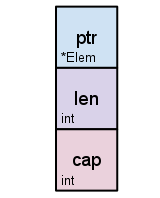
\includegraphics[scale=1]{slice-struct.png}
    \end{center}

    \begin{itemize}
        \item ptr wskazuje początek tablicy
        \item len jej długość
        \item cap jej pojemność
    \end{itemize}
\end{frame}

\begin{frame}[fragile]
    \frametitle{Slice III}
    Dzięki takiemu zabiegowi, slice dają nam ciekawe możliwości indeksowania:

    \begin{minted}[fontsize=\footnotesize]{Go}
        a := []int{1, 2, 3}
        b := a[2:]
        c := a[:1]
    \end{minted}

    Powyższe indeksowanie różni się od tablic. Tutaj nie mamy kopii tablicy, pracujemy
    wciąż na oryginale. Z tego powodu:

    \begin{minted}[fontsize=\footnotesize]{Go}
        a := []int{2, 3, 4}
        b := a[1:]
        b[0] = 4
        fmt.Println(a)
    \end{minted}

    Wypisze nam: \quotes{2, 4, 4}.
\end{frame}

\begin{frame}[fragile]
    \frametitle{Slice IV}
    Dzięki temu, że slice jest obiektem wskazującym na tablicę, Go nie musi 
    kopiować zawartości, tylko sam ten obiekt. Gdyby spojrzeć jak to wygląda
    pod spodem, to dostaniemy:

    \begin{center}
        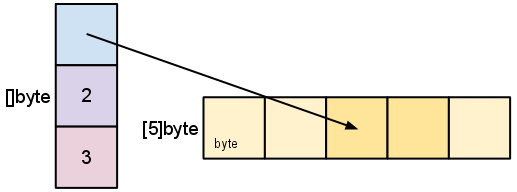
\includegraphics[scale=0.25]{slice-2.png}
    \end{center}

    Widać, że wyciągnięcie \quotes{kawałka} slice powoduje, że zmienia sie tylko
    obiekt definiujący slice.
\end{frame}

\begin{frame}[fragile]
    \frametitle{Slice V}
    Można by powiedzieć, że z wielkimi możliwościami przychodzi wielka odpowiedzialność.
    Tutaj w zasadzie pasuje powiedzieć, że przychodzą wielkie memory leaki.

    GoLang pracuje w oparciu o garbage collector. Można tutaj zrobić bardzo niemiłą rzecz,
    czyli:

    \begin{minted}[fontsize=\footnotesize]{Go}
        a := []int{2, 3, 4}
        b := a[1:]

        return b
    \end{minted}

    Kod wygląda ok, lecz generuje pewnego rodzaju memory leaka.
    
    Tablica pod spodem, jest trzymana w całości tak długo, jak istnieje przynajmniej jeden
    slice. Nie ważne, że ma on 1 element, a tablica 1000, GC nie wyrzuci zbędnych 999.
\end{frame}

\begin{frame}[fragile]
    \frametitle{Slice VI}
    Aby poradzić sobie z tym problemem, powstała funkcja \quotes{copy}:
    \begin{minted}[fontsize=\footnotesize]{Go}
        a := []int{2, 3, 4}
        b := make([]int, len(a[1:]))
        copy(b, a[1:])
        return b
    \end{minted}

    \begin{block}{Zamiana array na slice}
        Najłatwiejszy sposób zamiany tablicy na slice jest: \quotes{myArray[:]}.
        Utworzy on nowy slice, który w dodatku nie kopiuje tablicy pod spodem, lecz
        jej używa.
    \end{block}

    \begin{alertblock}{Uwaga!}
        Pomiędzy funkcjami najlepiej przekazywać slice, zamiast tablicy. Tablica
        jest przekazywana przez wartość, czyli jej kopia. Przy dużych tablicach
        może to chwile potrwać. Dlatego lepiej przekazać slice. 
    \end{alertblock}

    \begin{alertblock}{Uwaga 2!}
        Jeżeli mamy funkcję \quotes{func a(b int[])}, to nie przyjmie ona argumentu:
        \quotes{[3]int{1, 2, 3}}
    \end{alertblock}
\end{frame}


\section[Struktury]{Struktury}
\begin{frame}[fragile]
    \frametitle{Struktury}
    Struktura to definicja własnego wyglądu obiektu. Zawiera ona zbiór pól, jakie
    struktura ma zawierać.

    \begin{minted}[fontsize=\footnotesize]{Go}
        type MyStruct struct {
            FieldA int
            FieldB string
        }
    \end{minted}

    Warto pamiętać, że nazwy pól struktury także poddają się zasadzie prywatności ze
    względu na wielkość pierwszej litery.
\end{frame}

\begin{frame}[fragile]
    \frametitle{Struktury II} 
    Podstawowe poperacje na strukturze:

    \begin{minted}[fontsize=\footnotesize]{Go}
        type MyStruct struct {
            FieldA int
            FieldB string
        }

        myValue := MyStruct {
            FieldA: "A",
            FieldB: "B",
        }

        myValue2 := &MyStruct {
            "A",
            "B",
        }

        myValue == *myValue2 // true
        myValue.A = "A1"
        myValue2.B = "B"
    \end{minted}
\end{frame}

\begin{frame}
    \frametitle{Struktury III} 
    Należy pamiętać, że podawanie pól w strukturze jest opcjonalne przy tworzeniu.
    Najlepiej używać funkcji tworzących struktury.

    Przekazywanie struktury jako argument funkcji powoduje zrobienie jej kopii.
    Przy dużych strukturach zaleca się wskaźniki.

\end{frame}

\begin{frame}[fragile]
    \frametitle{Struktury IV} 
    Struktury nie mogą po sobie dziedziczyć. Jako symulację tworzy się pole anonimowe:
    
    \begin{minted}[fontsize=\footnotesize]{Go}
        type MyStruct struct {
            FieldA int
            FieldB string
        }

        type ExtendedStruct struct {
            MyStruct
            FieldC string
        }

        a := ExtendedStruct{
            MyStruct{
                FieldA: 87,
            },
            "C",
        }

        a.FieldB == a.FieldC
    \end{minted}
\end{frame}

\begin{frame}[fragile]
    \frametitle{Struktury V}
    Istnieje możliwość zdefiniowania struktury, która będzie posiadać własne metody.
    Metody w GoLangu przyjmują \quotes{receivera}, który może być wskaźnikiem.
    
    \begin{minted}[fontsize=\footnotesize]{Go}
    type MyStruct struct {
        FieldA int
        FieldB string
    }

    func (m *MyStruct) test () {
    }

    func (m MyStruct) test2 () {
    }
    \end{minted}

    Receivery, które nie są wskaźnikami, nie mogą modyfikować struktury.

    Zazwyczaj Go będzie dbać o poprawne tworzenie wskaźników w takiej strukturze.

    \href{https://github.com/golang/go/wiki/CodeReviewComments#receiver-type}{Polecam ten URL jeżeli nie wiesz który typ wybrać}
\end{frame}
    

\section[Mapa]{Map}
\begin{frame}[fragile]
    \frametitle{Map}
    Mapa pozwala na zapisywanie wartości typu \quotes{klucz: wartość}. Pod spodem jest
    zaimplementowana hashmap.

    W mapie jako klucz może być dowolny typ, który da się porównać.

    Mapę zapisujemy jako:
    \begin{minted}[fontsize=\footnotesize]{Go}
        var m map[string]int
    \end{minted}

    Mapa jest wskaźnikiem, dlatego też powyższy zapis spowoduje utworzenie zmiennej
    z wartością nil. Aby przypisać jej wartość, można użyć \quotes{make}

    \begin{minted}[fontsize=\footnotesize]{Go}
        m = make(map[string]int)
    \end{minted}
\end{frame}

\begin{frame}[fragile]
    \frametitle{Map II}
    Mapę można szybciej inicjalizować:

    \begin{minted}[fontsize=\footnotesize]{Go}
        m := map[string]int{}

        k := map[string]int{
            "a": 20
        }
    \end{minted}

    Operacje na mapie są proste:
    \begin{minted}[fontsize=\footnotesize]{Go}
        m["b"] = 50
        a := m["a"] // if not exists, returns zero value

        c, ok := m["c"]
    \end{minted}
\end{frame}

\begin{frame}[fragile]
    \frametitle{Map II}
    Z mapy można usuwać elementy za pomocą funkcji \quotes{delete}

    \begin{minted}[fontsize=\footnotesize]{Go}
        k := map[string]int{
            "a": 20
        }

        delete(k, "a")
    \end{minted}

    Oraz po mapie można iterować:
    \begin{minted}[fontsize=\footnotesize]{Go}
        for key, value := range k {
            
        }
    \end{minted}
\end{frame}

% rzutowanie

% interface są dla używających
% własne typy
\end{document}
